% !TEX root = ../thesis-example.tex
%todo: to describe the basic Magic Mirror idea, hardware and framework
%Magic Mirror framework: conception, software and hardware
\section{Magic Mirror framework} \label{sec:3-PPMM:MMC}
%the reason to choose anatomy learning for Magic Mirror conception
The Magic Mirror \cite{Grosjean1999} is a user interface technique that mimics a normal mirror and presents non-physical visual feedback in addition to the normally optical effect. Here the user stands in front of a screen and via a camera, the image of the user is shown on the screen such that it acts like a mirror. 
While previous systems have augmented objects onto the user, this system extends the Magic Mirror concept for medical education and rehabilitation. It creates the illusion that the user can look inside their own body. An depiction of this can be seen in \figurename{\ref{fig:3-MMC:Prototype}}. To achieve this visualization, the Magic Mirror augments the volume visualization of a CT dataset onto the user. 
To allow a correct augmentation of the medical data, the pose of the user is tracked. The Magic Mirror concept came out as a framework and it generates a personalized perception of the medical information for every user. In addition, the framework takes the user's natural gesture as input to create an interactive MR environment. 

Knowledge about human anatomy is an important issue for everyone working in the field of medicine. 
It is also an important part of the general education and relevant for many other professions related e.g. to health-care or sports. Human anatomy is very complex and it does not only involve knowledge about the single organ, but also about issues such as chemical processes, human motion and spatial relations inside the body. Therefore, teaching human anatomy is very difficult and often large effort is spent on teaching it e.g. by letting students perform dissection courses,\add{ creating illustrations and plastic models of anatomy} or by utilizing 3D computer graphics.
Our Magic Mirror framework is firstly employed to display anatomical structures overlaid onto the body of the user to intuitively teach human anatomy. 

\subsection{Magic Mirror prototype}
The augmented reality Magic Mirror prototype focuses on a few important organs of the abdomen, such as liver, lungs, pancreas, stomach, and bones.  
The system prototype has a mirror-like effect to the user by projecting a ``looking glass'' on the body and displays the skeleton of the user, rendered from CT data and anatomy 3D model (see \figurename{\ref{fig:3-MMC:Prototype}}). 
%The prototype of the Magic Mirror is largely based on a software framework that has been developed for HMD-based AR. 
The framework tracks users' movements using a depth camera and an algorithm to detect the pose of the user from the depth image. This is realized using the Microsoft Kinect which was originally developed to allow controlling computer games by motion. 
By using the Magic Mirror metaphor, the user is led to believe that he or she is able to look inside their own body. At the same time, medical information (CT, MRI data and a fully segmented dataset of cross-sectional photographs of the human body) are augmented in real-time. The current system also allows visualization of static anatomy on the user and offers a simple user interface to select CT, MRI or photographic slices \cite{Blum2012,Navab2012a}.
\begin{figure}
	\centering
	\includegraphics[width=0.9\linewidth]{figures/3-MMC/Figure1}
	\caption[The Magic Mirror prototype.]{The system prototype has a mirror-like effect to the user by projecting a ``looking glass'' on the body. By using the Magic Mirror metaphor, the user is led to believe that he or she is able to look inside their own body.}
	\label{fig:3-MMC:Prototype}
\end{figure}

\subsubsection{Hardware setup}
An illustration of the hardware setup can be seen in \figurename{\ref{fig:3-MMC:hardware:a}}. The first component of the system is a display device. In different setups of the system large TV screens or video projection onto a planar surface has been used. The second component is a color camera, which is mounted next to the display surface and which is looking at the user and perceive the visual information. The third component is a depth sensor which is placed next to the color camera and which has a similar field of view and viewing direction as the color camera to collect the user's skeleton information. 
The current system uses the Microsoft Kinect V1, which consists of a color and a depth camera that are assembled into one housing (see \figurename{\ref{fig:2-bg:kinect}} and \figurename{\ref{fig:3-MMC:hardware:b}}). The depth sensor is an infrared camera that uses structured light, which is emitted by an additional infrared projector to estimate depth values for each pixel. The user's skeleton and personal information can be generated from the Kinect sensor based on the machine learning.
The system employs the color camera to create a mirror-like effect to the user, and all the non-physical visual feedback is generated based on the user's skeleton and personal information via rendering the corresponding medical information onto the human body.

\begin{figure}
	\centering
	\subfloat[General Design]{\label{fig:3-MMC:hardware:a}
		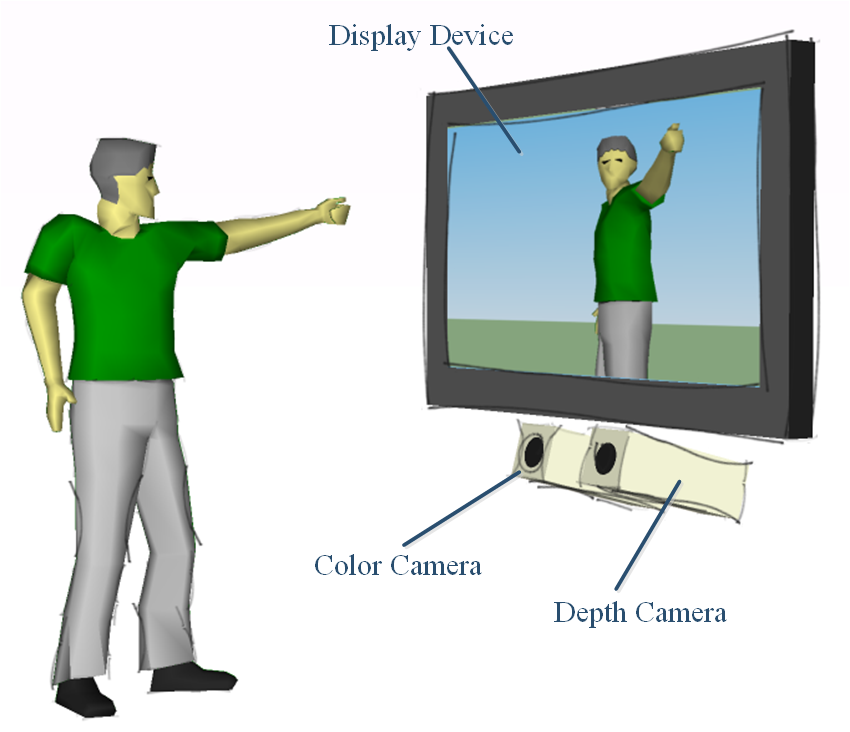
\includegraphics[width = 0.5\linewidth]{figures/3-MMC/GeneralSetup}
	}
	\subfloat[Current Implementation using Kinect]{ \label{fig:3-MMC:hardware:b}
		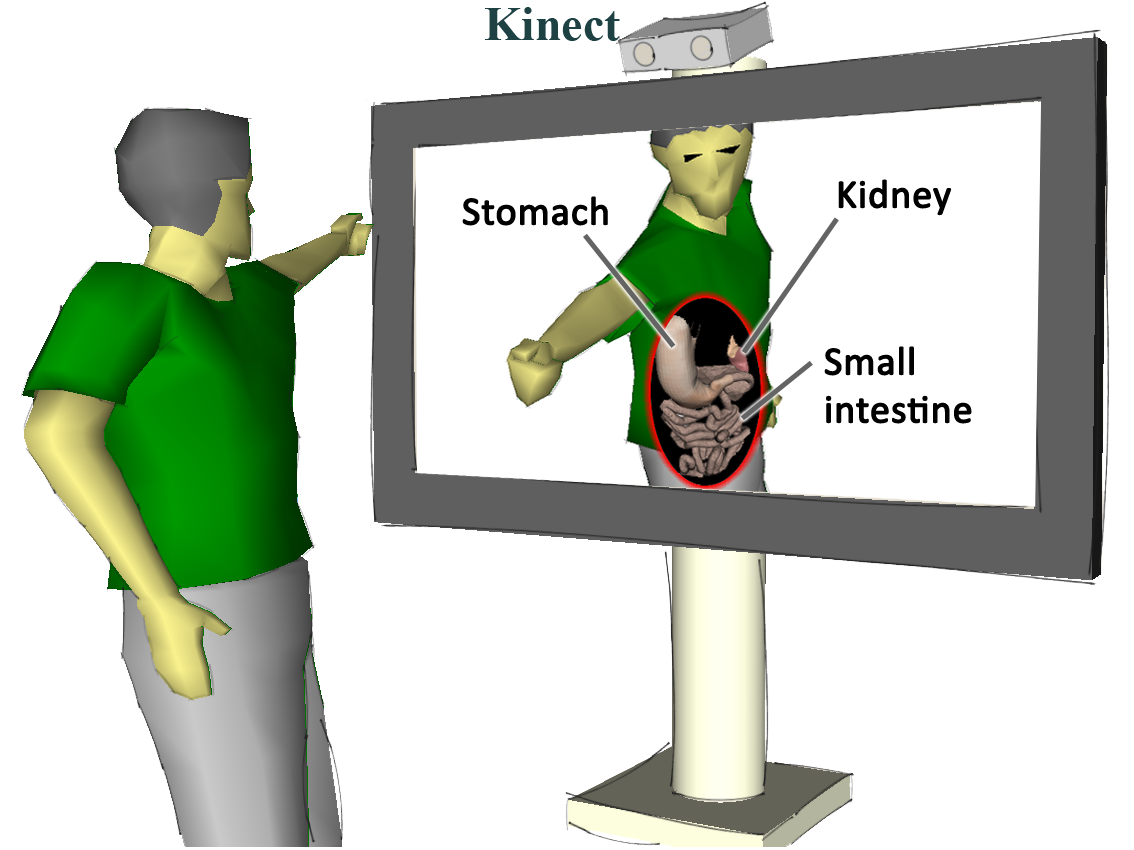
\includegraphics[width = 0.5\linewidth]{figures/3-MMC/mirracleIllustration}
	}
	\caption[Magic Mirror Hardware setup.]{Magic Mirror Hardware setup. (a) The system consists of a display, a color camera and a depth sensor. The color camera perceives the visual image, which is shown in the display to generate a mirror effect. The depth sensor observes the user and collects natural input for interaction with the system. (b) The color and depth camera are replaced by one Microsoft Kinect.}
	\label{fig:3-MMC:hardware}
\end{figure}

\subsubsection{Software framework}
The system framework of the prototype is illustrated in \figurename{\ref{fig:3-MMC:systemFramework}}.
To access the Kinect the system uses Microsoft Kinect SDK or OpenNI\footnote{\url{https://en.wikipedia.org/wiki/OpenNI}}, which is an open source software framework that allows retrieving color and depth images from the Kinect. The depth sensor is used for two purposes. First, the depth values are projected to the color image providing depth information for each pixel in the color image. Second, a skeleton tracking algorithm uses the depth image to track the pose of multiple joints of a user who is standing in front of the camera. For skeleton tracking the Magic Mirror uses NITE a software by PrimeSense that performs gesture recognition and skeleton tracking based on depth images. NITE can be used with the Kinect through the OpenNI framework.
\begin{figure}
	\centering
	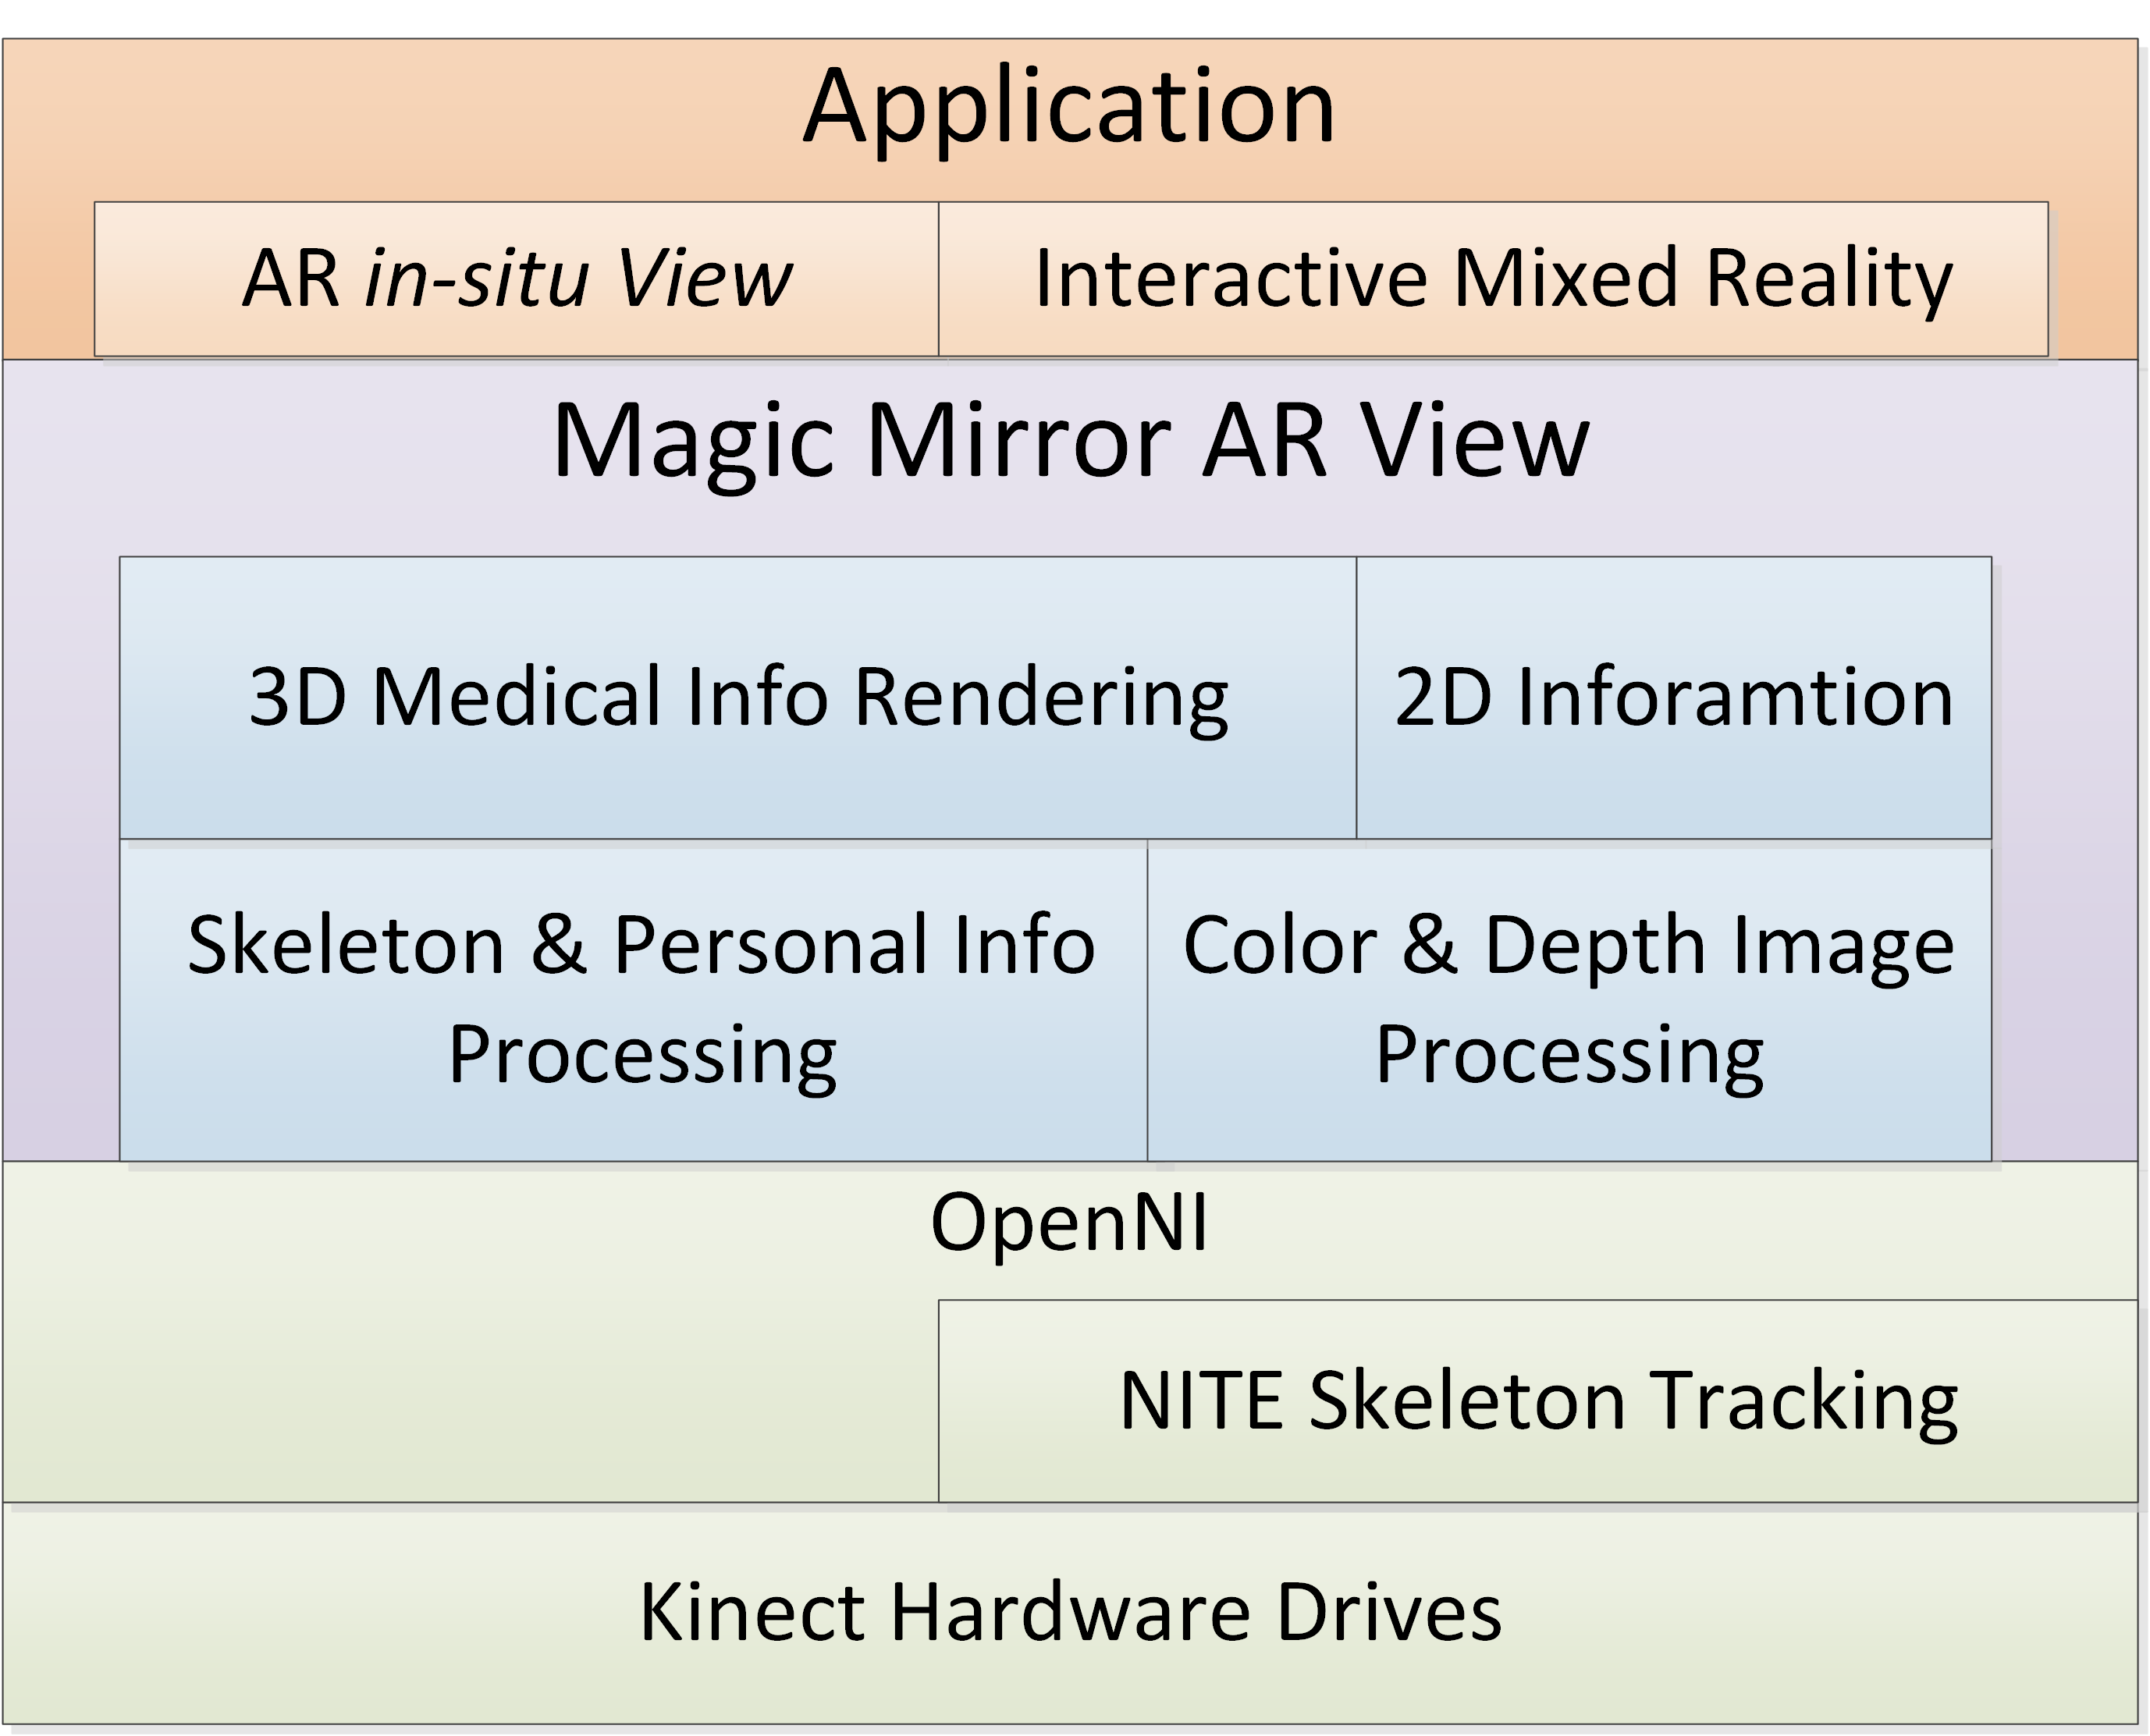
\includegraphics[width = 0.7\linewidth]{figures/3-MMC/SystemFramework}
	\caption[Magic Mirror system framework]{Magic Mirror system framework. The lowest two layers represent the open source library to access the Kinect raw image data and skeleton information. The middle layer is the modules used to create Magic Mirror AR view of the user. The top level is the application with basic system features.}
	\label{fig:3-MMC:systemFramework}
\end{figure}

The Magic Mirror AR view is based on the information perceived via Kinect and corresponding medical information. As shown in \figurename{\ref{fig:3-MMC:systemFramework}}, there are four modules:
%\textit{Skeleton \& Personal Information Processing}, \textit{Color \& Depth Image Processing}, \textit{3D Medical Information Rendering}, and \textit{2D Information} to generate the mirror-like effect and non-physical visual feedback.
\ul{Skeleton \& Personal Information Processing} is important to achieve personalized perception. 
\ul{Color \& Depth Image Processing} is the basic module to generate the mirror-like effect and merge the non-physical visual outcome. \ul{3D Medical Information Rendering} processes the corresponding 3D medical images or models and generates virtual elements for the Magic Mirror AR view and it can employ OpenGL and OpenGl Shading Language, and any other 3D rendering libraries, e.g. Coin3D. \ul{2D Information} includes window management and basic user interface elements, such as 2D text and image information, and it can be implemented using Qt.

The applications based on the \textit{Magic Mirror AR View} has two important features, \textbf{AR \textit{in-situ} view} and \textbf{Interactive Mixed Reality}. The blue rectangles represent the basic visualization functions of the system, which would be discussed in details later. The prototype system discussed in this section is a personalized Magic Mirror system for anatomy learning (see \figurename{\ref{fig:3-MMC:Prototype}). 
%It focuses on important organs of the thorax and abdomen and the bones. The system can currently provide MR \textit{in-situ} visualization, render skeleton from an original CT-volume, and showcase 3D models of organs. The sensor tracks the user positions in real-time, and contextual \textit{in-situ} visualization algorithms enable the augmentation of organs and bones directly onto the user body.

\subsubsection{Medical Information}
Aside from text and 2D atlas, 3D volumes and models are also important methodologies to represent medical information. The common way in medicine is to use 3D volumes, where we have one pixel or voxel for every point in 3D. This is the kind of data we get from CT or MRI. The other ones are polygonal or surface models, where only the surface (e.g. skin or the surface of the organ) is stored. For models that have been created for education often surface models are used because they look better.
While the system can use a CT or MRI scan, it doesn't make sense to acquire a CT or MRI scan of the user if it is not required for medical reasons. Therefore, we augment the medical volume from the Visible Korean Human dataset (VKH) \cite{Park2006} onto the user. This dataset consists of a CT scan, a MRI volume and a photographic volume which has been acquired by stacking up cryosections. 
Most CT and MRI medical images are saved in the DICOM standard, which is the format that is used in all hospitals. Unfortunately, most software for research does not support DICOM. The Magic Mirror system takes a ``\textit{$\ast$.MHD}'' file as the medical data. One drawback of the volume data is that the 3D dataset cannot be deformed in real-time. So if the user bends, this is not reflected in the visualization of the medical data and also movements of the limbs are not visualized correctly. While later, possible solutions to address this issue are discussed, for the current system, which focuses on the abdominal area, this is a minor problem.

Visualizing structures other than bones from the CT is more challenging. In a first attempt, the segmentation that is available for the CT volume was used to visualize different organs in the abdominal area. The quality of the visualization was low, as the segmentation does not have sub-pixel accuracy and transfer-functions on CT intensities cannot provide a visualization with realistic colors and textures of organs. Therefore instead of using the volumetric data, additional polygonal models were integrated. The Anatomium\footnote{\url{www.anatomium.com}} dataset provides polygonal models of many organs of the human body. A scene graph including multiple organs was extracted from the dataset. Using Coin3D this scene graph is augmented onto the user. The simultaneous visualization of bones from CT and a polygonal model of the small intestine is shown in \figurename{\ref{fig:3-MMC:Mirracle}}.
	
\subsection{Personalized perception and interaction} \label{sec:3:MMCInteraction}
To create a Magic Mirror AR view for anatomy leaning, special medical data should be selected from the database and transformed based on current user's personal information and interaction (see \figurename{\ref{fig:3-MMC:MedicalInfoFlow}}). Then the data is processed to generate the non-physical visual effect, merging with the mirror-like color image based on the depth information. The user learns anatomy knowledge via perception of the AR view of their own body. Interaction can also be performed by the user intentionally or unintentionally to control the  selection and transformation of the medical information, enabling an interactive AR view.
\begin{figure}
	\centering
	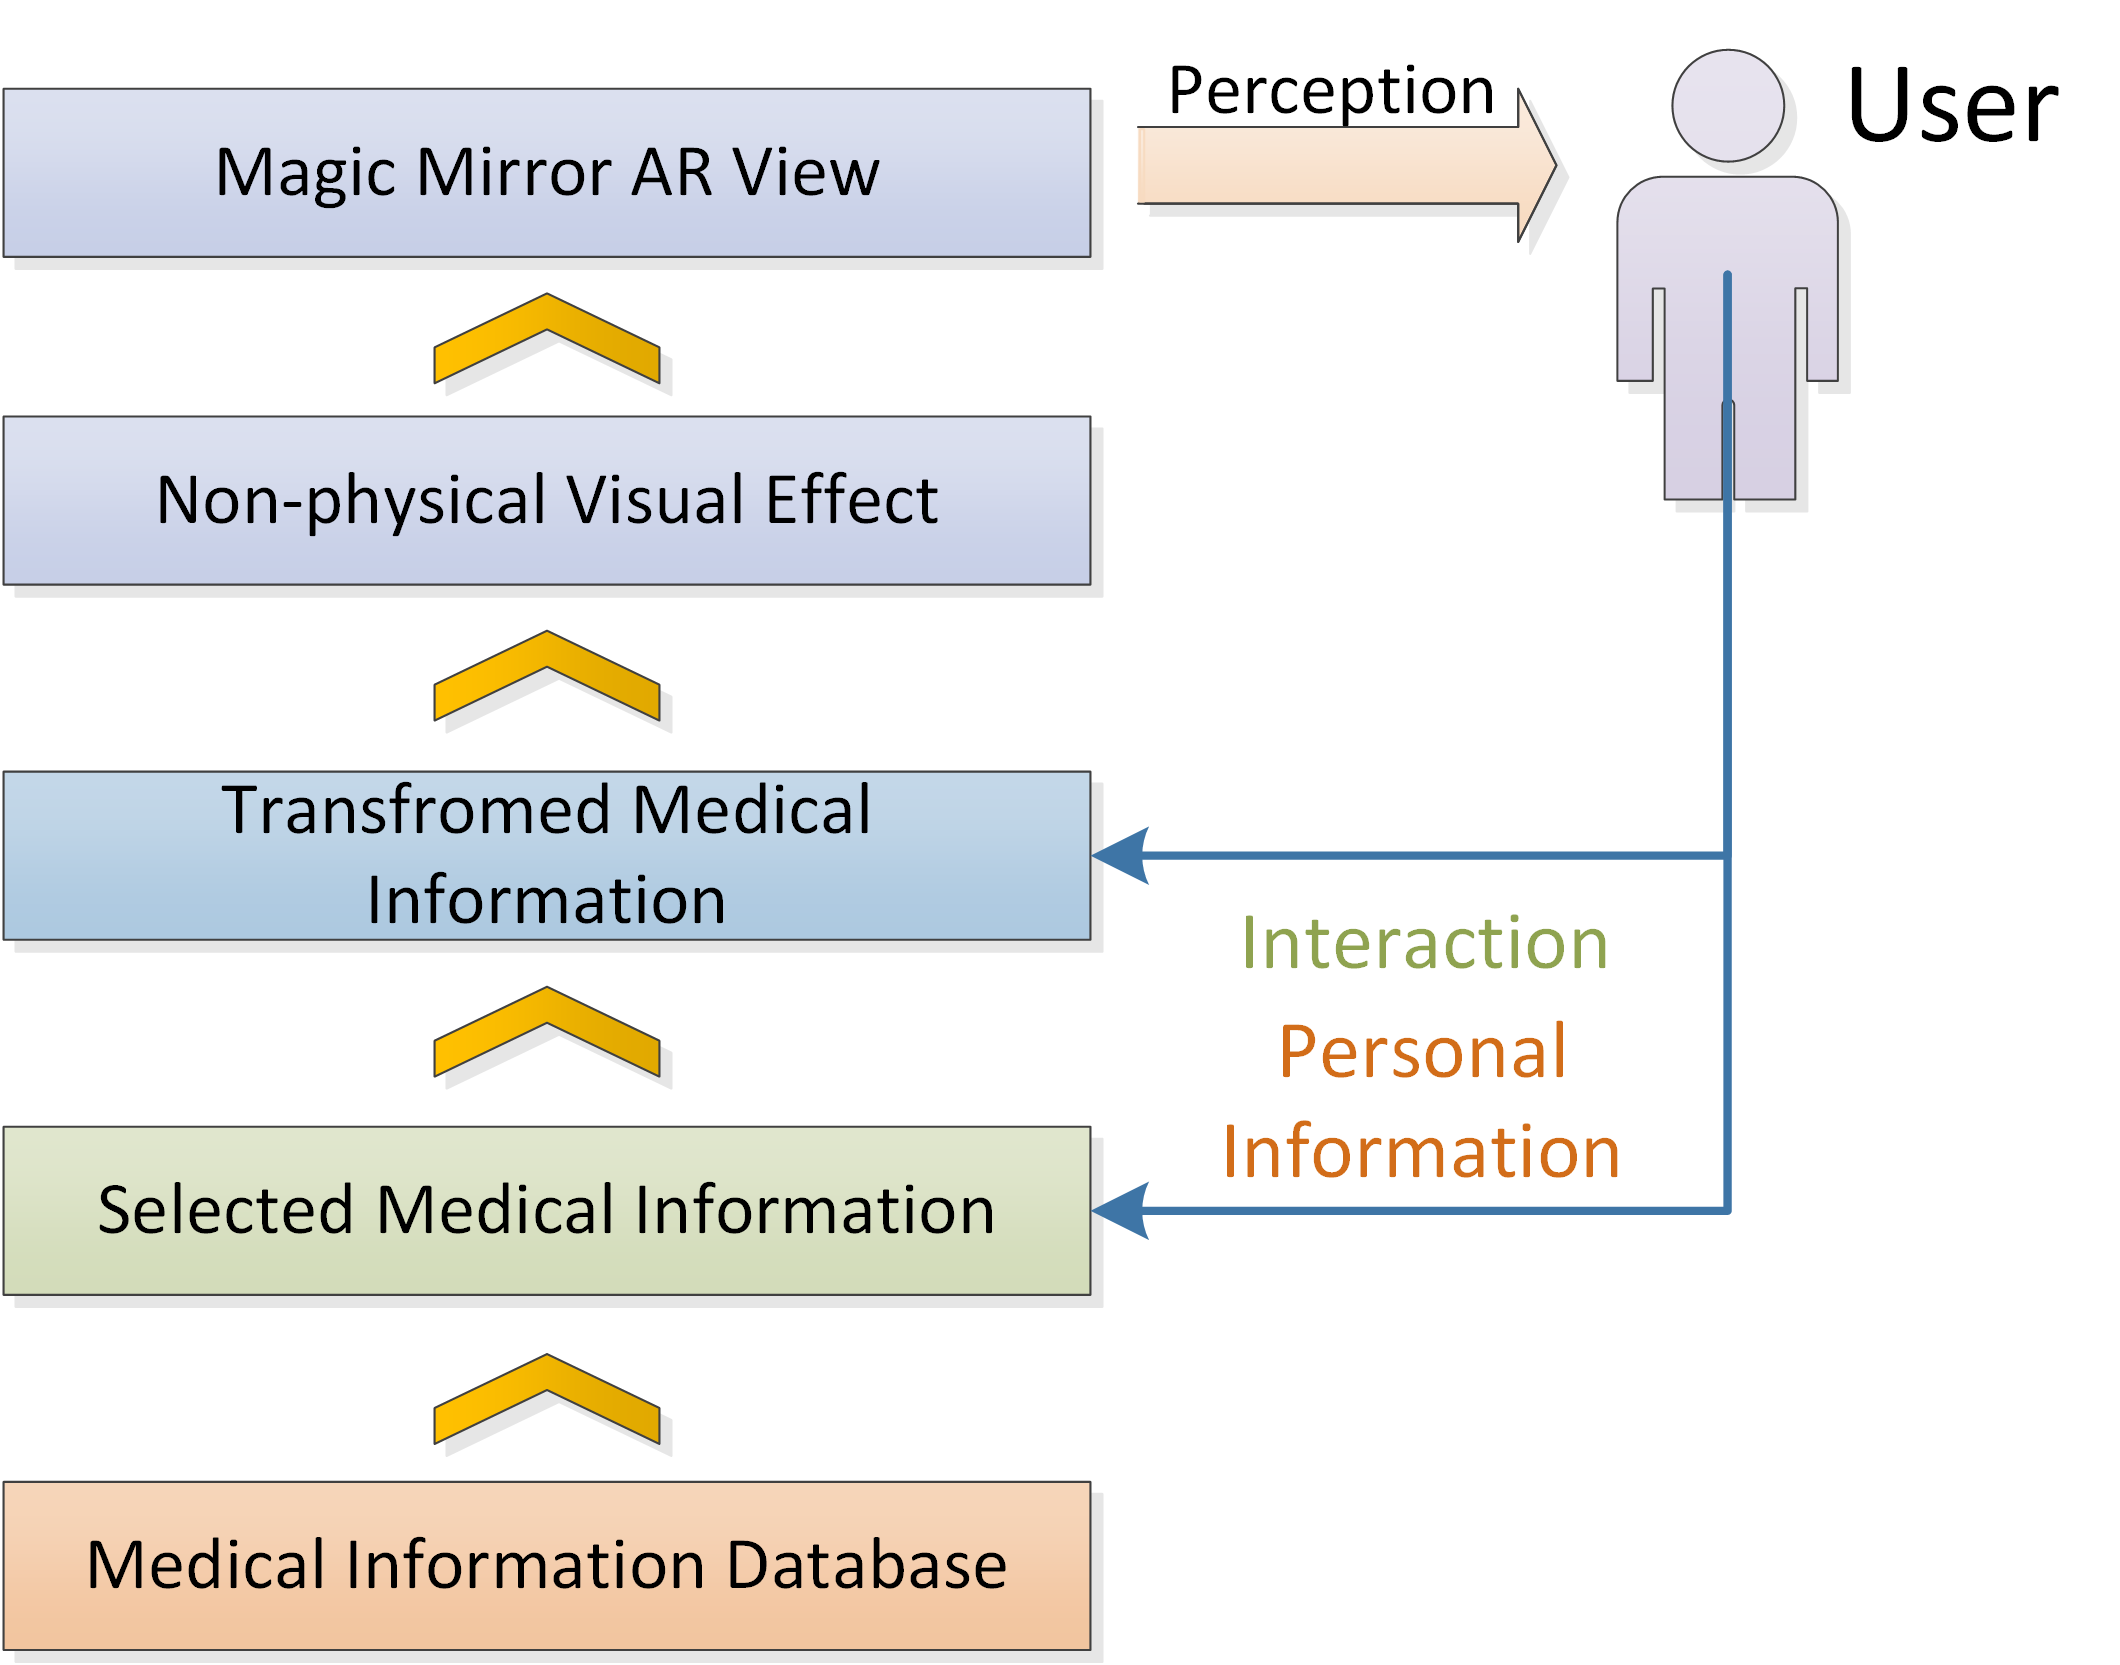
\includegraphics[width=0.7\linewidth]{figures/3-MMC/MedicalInfoFlow}
	\caption[Medical Information Flow]{For each non-physical visual effect, corresponding medical information is selected from the medical information database, transformed, and rendered according to the function setting and the user's interaction and personal information. Finally, the Magic Mirror AR view is generated.}
	\label{fig:3-MMC:MedicalInfoFlow}
\end{figure}

\subsubsection{Calibration of the user}
The skeleton tracking algorithm has to calibrate the user. For this, the user has to take a certain pose and hold it for several seconds. This calibration estimates the individual distances between joints for each user. This allows estimating the size of the user. The 3D volume and models are scaled to the size of the user and augmented onto the user.  
The NITE skeleton tracking algorithm, which is used in the Magic Mirror system, also requires the user to calibrate before the tracking works. In order to build a system that people can use without further instruction, we need to attract their attention and develop a self-explaining system. The NITE skeleton tracking provides a pixel map, where all pixels that belong to a person are labeled, before the user is calibrated. We use this to attract the attention of people passing by. As soon as someone walks into the field of view of the camera, that person is augmented with green color. The user has to take a calibration pose to become tracked. The system augments a silhouette of a person taking the calibration pose onto the display and asks the user to take the same pose. After calibration ends the system prints a message telling that a user has been recognized and the AR view can then be generated.

\subsubsection{AR in-situ visualization of human anatomy}
For a personalized visualization of organs the concept of a Magic Mirror is employed. The camera image is flipped horizontally and shown on the screen such that the user has the impression of standing in front of a real mirror. The system tracks all user movements using a depth camera and detects the pose of the user. Then, virtual elements are added to the image of the real scene. The augmentation context visualization \cite{Bichlmeier2007} is used, such that the virtual objects are only seen through a circular focus window (see \figurename{\ref{fig:3-MMC:Mirracle}). This leads to a better perception of depth, compared to a simple augmentation of the whole CT. 
By using the Magic Mirror metaphor, the user is led to believe that he or she is able to look inside their own body. At the same time, different medical information (CT data and a fully segmented dataset of cross-sectional photographs of the human body) can be displayed \cite{Blum2012}. For visualization of the bones a transfer function is used as bone can be distinguished easily in the CT volume based on the voxel intensities. For some applications where CT dataset of the user is available, it can directly augment the CT dataset onto their own body to improve the perception.
\begin{figure}
	\centering
	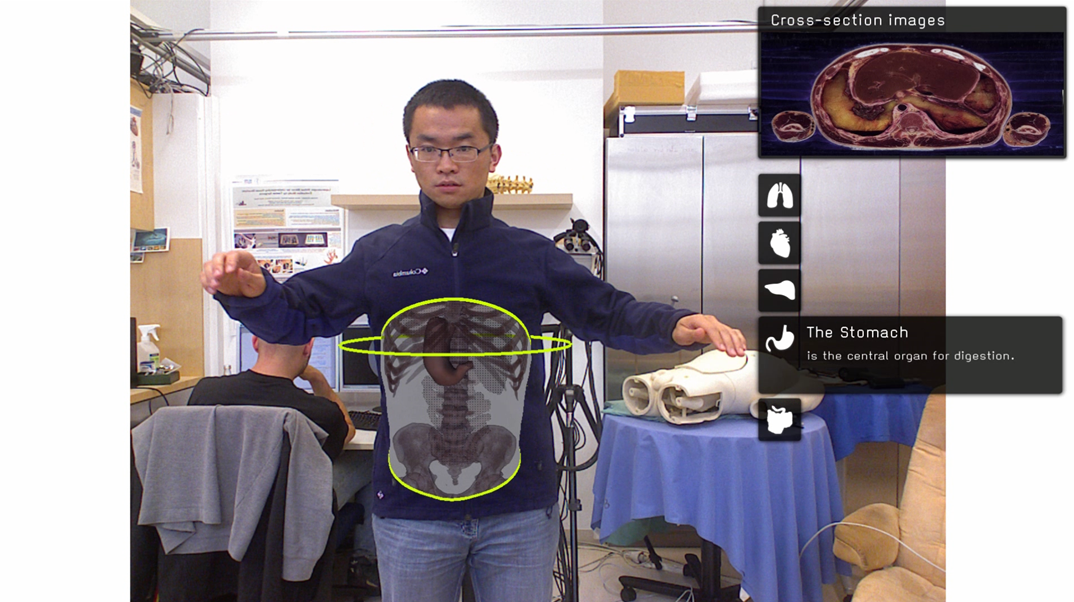
\includegraphics[width=0.9\linewidth]{figures/3-MMC/Mirracle}
	\caption{Magic Mirror Demo. The AR \textit{in-situ} visualization of human anatomy in the prototype Magic Mirror demo.}
	\label{fig:3-MMC:Mirracle}
\end{figure}

\paragraph{Presentation of additional medical information}
In addition to the AR \textit{in-situ} visualization of anatomy, the system still has to show more detailed information via text, images and 3D models. To achieve this, the system switches to a mode, where the whole screen is used to display additional information about anatomical structures, such as the 2D slices from the CT or photographic volume.
Therefore, the system can switch to the 2D or the 3D models mode as needed, and both 3D view or 2D information can be displayed to improve the perception of the medical information.

\subsubsection{Natural user interaction}
All the body movements are tracked and can be directly employed for the interaction. Arm and hand gestures are used to perform interaction in the Magic Mirror MR environment.

\paragraph{Relocating the see-through window}
The \textit{see-through} window plays an important role in creating the personalized \textit{in-situ} visualization of the anatomy.
As shown in \figurename{\ref{fig:3-MMC:NUI:a}}, the window position is controlled by the hand position. A user specific offset vector is added to the left hand joint to calculate the window position. This interactive function motivates the user to learn where the interesting organ is. For public demos for children, we limited the window position in one dimension (see \figurename{\ref{fig:3-MMC:Mirracle}) and the user moves up or down to change the window position to show different organs in the corresponding planes.
	
\begin{figure}
	\centering
	\subfloat[Relocating \textit{see-through} window]{ \label{fig:3-MMC:NUI:a}
		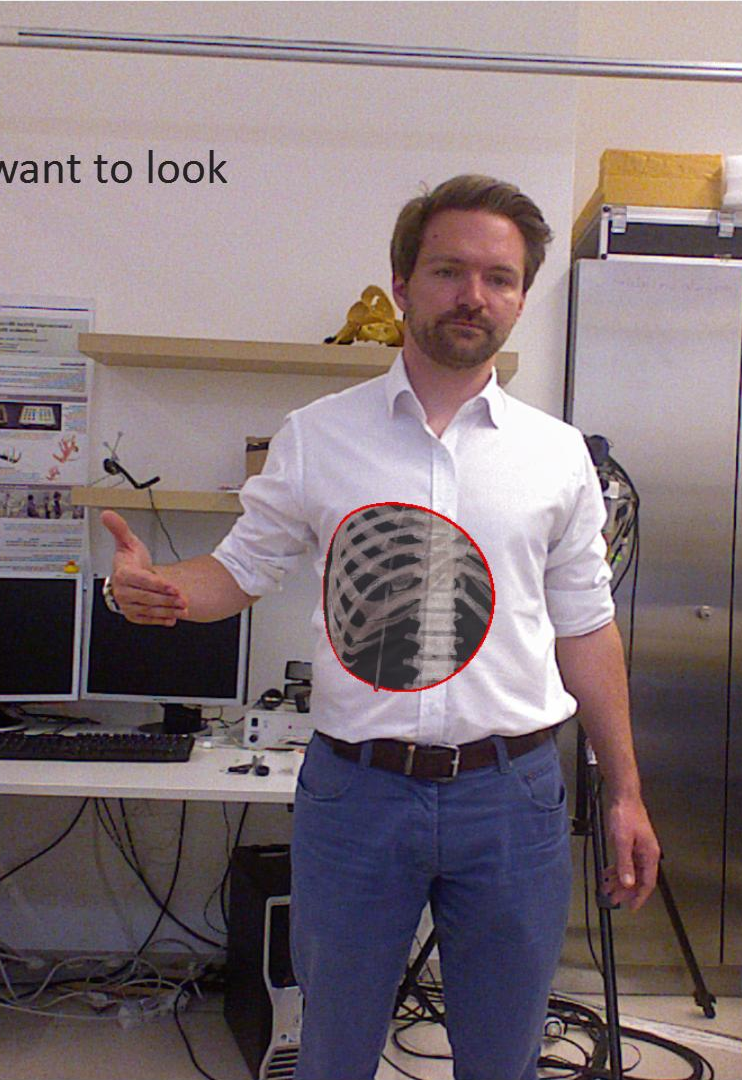
\includegraphics[height = 7cm]{figures/3-MMC/ChooseWindow}
	}
	\subfloat[Gesture-based interaction for slices]{\label{fig:3-MMC:NUI:b}
		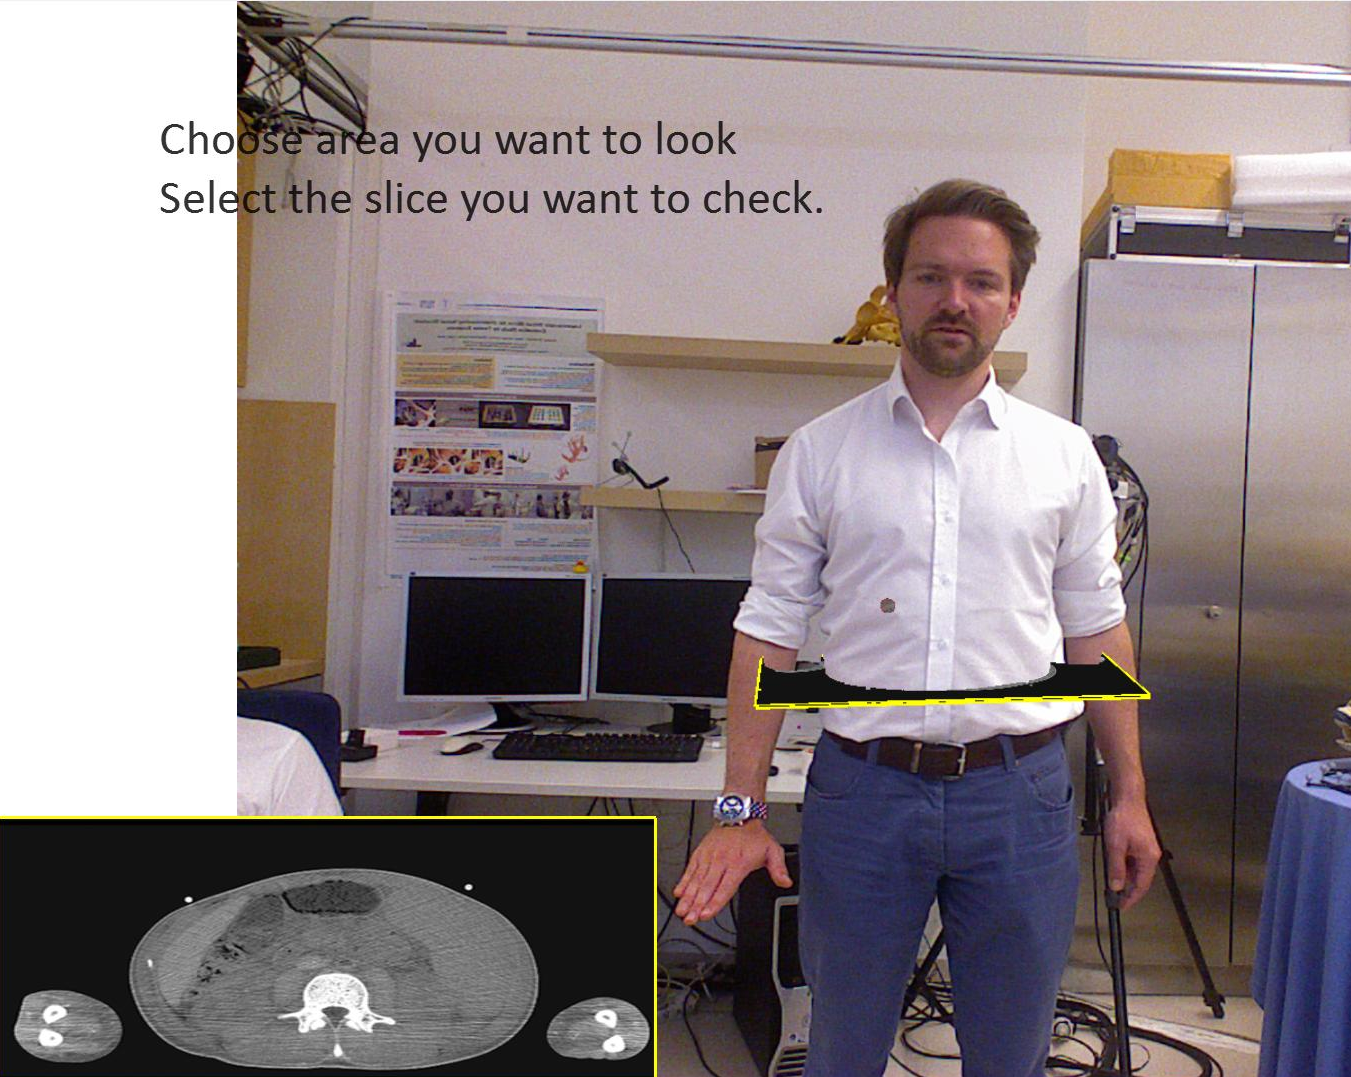
\includegraphics[height = 7cm]{figures/3-MMC/slicing}
	}
	\caption[Natural User interaction]{Arm and hand gestures can also be used to perform interaction with the Magic Mirror AR view. (a) The user can move the hand to relocate the \textit{see-through} window. (b) When the system is in the transverse slice mode, the user could move their hand up or down to choose the interesting slice image. }
	\label{fig:3-MMC:NUI}
\end{figure}
\paragraph{Gesture-based interaction for slices} A volume can be seen as a stack of transverse slices starting from the top and going to the bottom. Usually medical volumes are checked slice by slice to get the desired information. The current slice is depicted on one corner of the monitor while a yellow circle or rectangle is augmented onto the user depicting the slice plane.
The user can move their hand up or down to choose the interesting slice image (see \figurename{\ref{fig:3-MMC:Mirracle} and \figurename{\ref{fig:3-MMC:NUI:b}) when the system is in the transverse slice mode. It is similar for the sagittal slice mode. The system can easily switch slices between the CT and the photographic volume.
		
There is a trend toward competency-based education in medicine. Instead of defining a curriculum, learning outcomes are defined. Students have to fulfill these learning outcomes. The advantage of competency-based education is that all students will have the same competency in the end. A student who is less skilled has to take more time to learn than a student who already has good skills. One requirement for this is that the students have to be able to educate themselves until they reach the required competency. 
%We plan to use the AR Magic Mirror system both to allow them to do training and to test whether a learning outcome has been met. 
This framework can be made easily available to them so that they can use it for training and testing at any time.
	
\subsection{Evaluation of the framework}
The current system allows visualization of static anatomy on the user and offers a simple user interface to select CT or photographic slices. Demos of the prototype have been given on various public occasions. Medical doctors (MD) from physiotherapy, anatomy, radiology, sports medicine, children's medicine, and medical teacher and science centers are interested in using such a system in education of medical students and pupils. 
As an augmented reality anatomy learning application, system usability are very important prior to its translation in classroom. We undertook one user study involving first year medical students to verify the learning potential and acceptability of our technology as a compliment to atlas textbooks in classroom.

\paragraph{Learning Scenario} A list of questions are developed by the medical partners. Each question asks for the location of an anatomical structure. 
In the first step the student has to position the focus window at the correct location via the function ``Relocating the see-through window''. After positioning the window, the distance to the actual position of the structure is computed. If the distance exceeds a threshold it is considered as wrong. In this case the student has to reposition the focus window. When the correct position has been selected, the focus window is fixed and another mode is activated where a more fine grained selection is possible using ``Gesture-based interaction for slices''. 
In each question either one or more of the correct slices along the three directions have to be found. 
%After a set of questions are answered, a score is presented, which is based on the number of tries and the time a student required to find the correct slices.

\paragraph{Participants:} 72 medical students from the Anatomische Anstalt der Ludwig-Maximilians-Universit\"at M\"unchen, having an age range between 21yrs and 28yrs, were enrolled in this study. The distribution of gender was 38 male and 34 female. Their medical experience was: 50 participants did not have any expertise, 8 had paramedic training, 5 with healthcare training, and 9 with some other degree (e.g. biology, chemistry, and therapy). 

\paragraph{Analysis:} Responses to questions were based on a four point Likert Scale: (1) \textit{strongly disagree}, (2) \textit{disagree}, (3) \textit{agree}, and (4) \textit{strongly agree}. For statistical analysis, the response categories were reduced to Yes/No: Yes (\textit{agree} + \textit{strongly agree}); No (\textit{strongly disagree} + \textit{disagree}).

The study procedure involved every participant to use the personalized Magic Mirror system for 15 minutes and try all available system functions. Participants were then asked to assess the learning potential of the technology by responding to the following questions:
\begin{itemize}
	\item[Q1-] is the system helpful for anatomy learning?  
	\item[Q2-] do you like to use the Magic Mirror? 
	\item[Q3-] is the presentation and visualization of the CT volume acceptable? 
	\item[Q4-] do you like the AR view of 3D human anatomy? 
	\item[Q5-] what other information would you want to see from the 3D rendering? (Open question)
\end{itemize}
Frequencies (F) and percentages (\%) of response on the first four questions are given in \tablename{\ref{tb:3-MMC:userStudy}}. The questionnaire, focused on motivation and perception of the participants, showed statistically significant differences for all the questions. Percentages confirmed how the students accept this Magic Mirror system for anatomy learning.
\begin{table}
	\caption[User study with fresh medical students]{Frequencies and percentages of response of the medical students about the AR system.}
	\centering
	\label{tb:3-MMC:userStudy}
	\scriptsize
	\begin{center}
		\begin{tabular}{ccccccccc}
			\multicolumn{1}{c}{\space} & \multicolumn{2}{c}{\textbf{Q1}} & \multicolumn{2}{c}{\textbf{Q2}} & \multicolumn{2}{c}{\textbf{Q3}} & \multicolumn{2}{c}{\textbf{Q4}} \\
			\hline
			\space & \textit{F} &\textit{\%}& \textit{F} &\textit{\%}& \textit{F} &\textit{\%}& \textit{F} &\textit{\%} \\
			Yes & 62 & 86.1 & 60 & 83.3 & 68 & 94.4 & 66 & 91.7 \\
			No & 10 & 13.9 & 12 & 16.7 & 4 & 5.6 & 6 & 8.3 \\
			\hline
		\end{tabular}
	\end{center}
\end{table}

The results of question 5 are depicted in \tablename{\ref{tb:3-MMC:question5}. They indicate that the participants would eventually like the current Magic Mirror system to evolve to one that includes the visualization of complex anatomy models such as the vascular system, relations between different organs, extremities, etc. 
\begin{table}
	\caption[3D anatomy expected]{Frequencies and percentages of new 3D anatomy expected by the 72 medical students}
	\centering
	\label{tb:3-MMC:question5}
	\scriptsize
	\begin{center}
		\begin{tabular}{ccc}
			%\hline
			New 3D rendering functions & \textit{F} & \textit{\%} \\
			\hline
			vascular system &	19 &	26.4 \\
			relationship between different organs&	13	&18.1\\
			extremities &	10&	13.9\\
			landmarks&	6&	8.3\\
			static AR view with their body&	6	&8.3\\
			head/brain	&5	&6.9\\
			muscle&	5&	6.9\\
			others&	5&	6.9\\
			\hline
		\end{tabular}
	\end{center}
\end{table}

\subsection{Conclusion}
This section presents a personalized AR Magic Mirror framework and a prototype for anatomy education.
The prototype system creates a MR environment, which is certified useful for anatomy learning, and the majority of the medical students accepted the learning potential of the technology. 
The academic methodologies must be changed according to the advances of new technologies, but there is still a long way for this. 
Considering the benefits of the personalized and interactive AR system for motivation and perception of anatomy learning, new technologies can additionally be helpful to facilitate autonomous learning and secondarily to reduce laboratory material and instructor costs. Together with the anatomy community, we hope to initiate such discussions in integrating exciting user-specific and gaming concepts within curricula via new anatomy learning systems. 

%It was originally suggested to us that our system would have much more of an impact for medical education if it were to be translated today in medical schools and anatomy classrooms. As such, with the help of our partner and anatomy professor, we deliver the improved AR Magic Mirror to two anatomy classes within the Anatomy Department of the Ludwig Maximilian University (LMU) Medical School, Munich, Germany. 
%The anatomy professors made it clear that the proposed system is exciting, but has to go beyond state-of-the-art technology to be truly useful for education. Our participants stressed the importance of visualization of anatomy that can change dynamically resulting from the actions of the user moving the body. Furthermore, more advanced user interactions like the use of gaming elements would be required to make the use of the system for learning and rehabilitation tasks more interesting.